%%
% Template for using the IEEEtran documentclass
% Uses onecolumn journal style with 10 pt font
%%
\documentclass[journal,onecolumn,twoside,10pt]{IEEEtran}

%% Include any other packages you want here.
\usepackage{lipsum} % Generate dummy text.
\usepackage{graphicx} % Enable graphics

% "Double" spacing
\linespread{1.6}

% paper title
% can use linebreaks \\ within to get better formatting as desired
\title{Sample Document for CprE 308}

% Author Name
\author{Your~Name} 

%% Header info.  First part for page one and even, second for odd after first.
\markboth{CPRE 308 FINAL PROJECT, SPRING 2014}
{LAST~NAME: TITLE}

% Begin document
\begin{document}

% Include title information
\maketitle

% Use the input command to include other files (notice we don't need the extension)
% Feel free to add as many files as necessary.

\begin{abstract}
Address space layout randomization (ASLR) is a security measure that many popular operating systems use to slow down and lessen the chances of success of buffer overflow attacks. This method randomizes key parts of a program’s address space to make it more difficult for an attacker to find an exploited function in memory. Because the memory locations are randomized, it makes it much more difficult for an attacker to guess where the areas are located.

In this paper, I will be analyzing the background, implementation, and effectiveness of ASLR. I would like to understand the evolution of ASLR as it progressed from an experimental idea to a method implemented in all major operating systems. My goal will be to gain a strong understanding of the concepts and methods behind a modern implementation of randomizing address space layouts. Though I will mention a few common ASLR implementations, I will focus mainly on the implementation in the Linux kernel. Once I have set up a strong basis for ASLR, I will analyze how effective this method is for thwarting attackers. In addition, I will weigh the performance costs of implementing ASLR on a system when compared to a system without ASLR, or even a partial implementation.
\end{abstract}

\section{Introduction}
\label{s:intro} % This declares a label so you can reference the section elsewhere.

\IEEEPARstart{A}{ddress} space layout randomization (ASLR) is a security measure that many popular operating systems use to slow down and lessen the chances of success of buffer overflow attacks. This method randomizes key parts of a program’s address space to make it more difficult for an attacker to find an exploited function in memory. Because the memory locations are randomized, it makes it much more difficult for an attacker to guess where the areas are located.
\\
In this paper, I will be analyzing the background, implementation, and effectiveness of ASLR. I would like to understand the evolution of ASLR as it progressed from an experimental idea to a method implemented in all major operating systems. My goal will be to gain a strong understanding of the concepts and methods behind a modern implementation of randomizing address space layouts. Though I will mention a few common ASLR implementations, I will focus mainly on the implementation in the Linux kernel. Once I have set up a strong basis for ASLR, I will analyze how effective this method is for thwarting attackers. In addition, I will weigh the performance costs of implementing ASLR on a system when compared to a system without ASLR, or even a partial implementation.


\section{Background}
\label{s:background} % This declares a label so you can reference the section elsewhere.

To understand why address space layout randomization is important, it is necessary to make sense of the kinds of attacks it helps mitigate. Buffer overflow attacks are the main class of attacks that ASLR tries to prevent. A buffer overflow happens when the data being entered into a buffer is larger than the allocated buffer space. The data typically then is placed in the adjacent memory locations to the buffer. It is usually unknown what is in those overwritten memory locations. An example of this bug can be seen in Fig. 1. In this example, a string of length eight is placed into a buffer of length six. Since the input data is longer than the buffer, the extra data is overflowed into the following memory locations. In this instance, the following memory locations make up another variable.

This failure to check the bounds on the input causes a bug. A malicious attacker could potentially use bugs like these to overwrite memory in their favor. One common method to exploit these bugs is to overwrite the return address on the program’s stack. This is called a stack buffer overflow. When an exploited function returns, it jumps to the address in the return address specified by the stack. The program will begin execution somewhere other than the intended place. There are many variations of the buffer overflow attack, but this demonstrates how severe these bugs are.

The idea behind ASLR was first implemented by Memco Software in 1999~\cite{yarom1999method}. ASLR first showed up in Linux as part of PaX project in 2003~\cite{paxdocs}. Since then, several other operating systems have implemented versions of ASLR, including Windows~\cite{msexploitmitigation} and Mac OS X~\cite{applesecurity}. This demonstrates the importance of this security feature in modern operating systems.

\section{Implementation}
\label{s:implementation} % This declares a label so you can reference the section elsewhere.

To understand how address space layout randomization works in Linux, one must first know how an address space is laid out for a particular process. There are three main parts of a process’s address space: text, data, and stack \cite{memorylayout}. The text space holds the executable code of the process. This is a static, read-only block of memory. Next, there is the data segment. This section stores the program’s variables, in particular the primitives, arrays, and strings that the programmer declared. Finally, there is the stack, which is a Last-In-First-Out (LIFO) structure that contains information about the program’s execution subroutines. The text segment is traditionally at the bottom of the address space, followed by the data, with the stack located at the end of the allocated address space. The layout can be seen in Figure \ref{f:memory_layout}.

\begin{figure}
\centering % Make it center
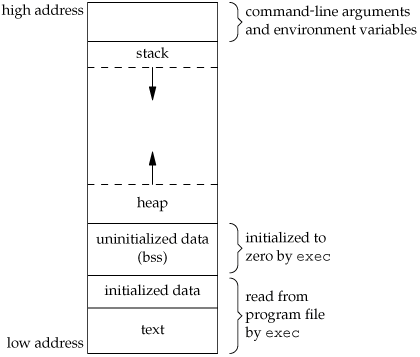
\includegraphics[width=0.5\textwidth]{figures/Memory-Layout.png}
\caption{The layout of a process's memory in Linux \cite{memorylayout}}
\label{f:memory_layout}
\end{figure}

While the predictability of the locations of these parts of the address space would seem convenient, it can assist serious security attacks, such as the one detailed above. ASLR randomizes key parts of the virtual address space for a process. There are differing and weaker variations to this system. Because ASLR can introduce performance penalties on systems with smaller memory sizes, the security benefits may not always outweigh the performance loss. Different operating systems will sometimes only implement ASLR for crucial security components, for example. The level of randomization that occurs can be chosen when compiling the Linux kernel using the randomize\_va\_space sysctl file. There are three main options: 0 for no randomization, 1 for randomization of the mmap base, stack, and VDSO page, and 2 for complete randomization, which includes the heap. \cite{kerneldocs}

In a nonrandomized process, the location of the stack is in the same place on every execution. However, in an operating system with ASLR enabled, a process’s address space is randomized at runtime, and therefore the stack will be in a different place every time the process is created. The kernel acts as a middle-man and keeps track of where the randomized pieces are located. The source for the function in the Linux kernel that is used to randomize the addresses is shown below. It’s main purpose is to “return a start address such that a <range> with size 'len' starting at the return value is inside in the area defined by [start, end], but is otherwise randomized.” \cite{randomc} The result is that the stack is now in an unknown location, significantly reducing the effectiveness of stack buffer overflow attack.

\begin{lstlisting}[caption=Source for the range randomization function]
unsigned long randomize_range(unsigned long start, unsigned long end, unsigned long len)
{
	unsigned long range = end - len - start;

	if (end <= start + len)
		return 0;
	return PAGE_ALIGN(get_random_int() % range + start);
}
\end{lstlisting}

\section{Effectiveness}
\label{s:effectiveness} % This declares a label so you can reference the section elsewhere.

It is useful to analyze what impacts ASLR has on any given system. While ASLR has security benefits, it can have an impact on performance as well, so there are tradeoffs. In particular, it’s important to analyze how effective ASLR is thwarting attacks, how it can be broken or weaken, and the overhead associated with it.

The basis for the security effectiveness of ASLR depends upon the chance of an attacker guessing the randomized locations. To decrease the likelihood of a successful attack, the search space for a guess must be increased. The search space increases when there are more bits of entropy in the random number generation. If n is the number of bits of entropy available, then $2^n$ represents the total number of possible addresses. This number increases very quickly as entropy increases. For a 32-bit system, the number of bits of entropy is 16-20 bits. This leaves a relatively small search space that could easily be brute forced in a small amount of time with modern computing. Realistic implementations, such as PaX, have methods of preventing brute forcing, however. With the adoption of 64-bit architectures, the number of entropy bits increased to around 48 bits, making brute force infeasible.

When implemented perfectly, ASLR is a sound defense. Unfortunately if the implementation or some supporting code has a vulnerability or bug, ASLR can be bypassed. As previously stated, brute force may be possible if the conditions are correct, however this relies on a relatively small address space. The goal to getting past ASLR would be to exploit a bug in which the code leaks the starting memory address of a randomized memory segment. One common way that the address of a pointer is leaked is through a format-string attack. \cite{bhatkar2003address} An attacker uses the printf function or one of its variants where a input string is placed directly in the format-string parameter. The attacker can then use the \%n or \%d identifiers to output a random address on the stack. Using this, the attacker can sometimes find out the location of the stack or heap and use a more traditional exploit such as a buffer overflow. An information disclosure like this is the main way to bypass ASLR. There are other ways, but they rely on very rare bugs.

\begin{lstlisting}[caption=A dangerous printf statement][h]
printf(message);
\end{lstlisting}


Performance impacts differ based on the architecture and memory segment. On Linux, the performance hit can be as significant as 26\% for a 32-bit machine. \cite{payer2012too} The main cause for this is the requirement that executables must be compiled as position-independent in order to be compatible with ASLR. A position-independent executable is essentially a binary that is modified so that it can be run in any number of places in memory. This operation is very CPU register heavy and therefore causes significant performance losses for 32-bit architectures. On the other hand, since 64-bit architectures have more registers, ASLR has an almost negligible performance impact. It is interesting to note that the Windows implementation of ASLR suffers a negligible impact due to its method of randomization, which is at link-time rather than compile time.

\section{Conclusion}
\label{s:conclusion} % This declares a label so you can reference the section elsewhere.

Overall, address space layout randomization is a major benefit to any operating system. ASLR is an excellent security measure that thwarts potentially crippling attacks such as stack and buffer overflow attacks. By concealing the locations of a process’s key memory segments, it minimizes the probability of an attack succeeding. The probability decreases as the search space of the randomization increases, which makes 64-bit architectures perfect for this protection. In the right scenarios, ASLR has minimal performance costs.

During this study, I explored a powerful security feature that is implemented in almost all modern operating systems, even mobile ones. I had the chance to explore some common attacks on an operating system and the vectors in which they occur. Prior to my research, I was aware of what buffer overflows were, but was not familiar with how they could be used to violate a system’s intended use. This was a very interesting and useful project to engage in.


%% Include the bibliogrhy, using the IEEEtran style.
\bibliographystyle{IEEEtran}
\bibliography{reference} % Use bib information from reference.bib

% that's all folks
\end{document}
